\section{How to use Google Play} \label{Sprint4_SecHowToUseGooglePlay}
\textit{This section will describe how to use Google Play.}

To use the administrative side of Google Play you first and foremost need to be logged in at: https://play.google.com/apps/publish using an adminestrative account.

When logged in you have access to a list of the currently published apps sorted alphabetically on their name (the title of the app). The list also shows the current version, the rating, and when the apps were last updated, as well as a few other pieces of information.

When clicking on the name of an app, you are taken to the shop description, where you can change the description of the app and the various screenshots being used when the app is presented in Google Play. On Figure \ref{OverviewGooglePlay} an overview of the most important tabs is given. These include: the APK-tab (1), where version management is handled; the shop description-tab (2); the content-classification-tab (3), where the content declaration can be changed, see Section \ref{Sprint4_SecContentClassification}; and the price and distribution-tab (4), where the app’s availability can be changed. In addition to this, there are other more self-explanatory tabs.

\begin{figure}[H]
	\centering
	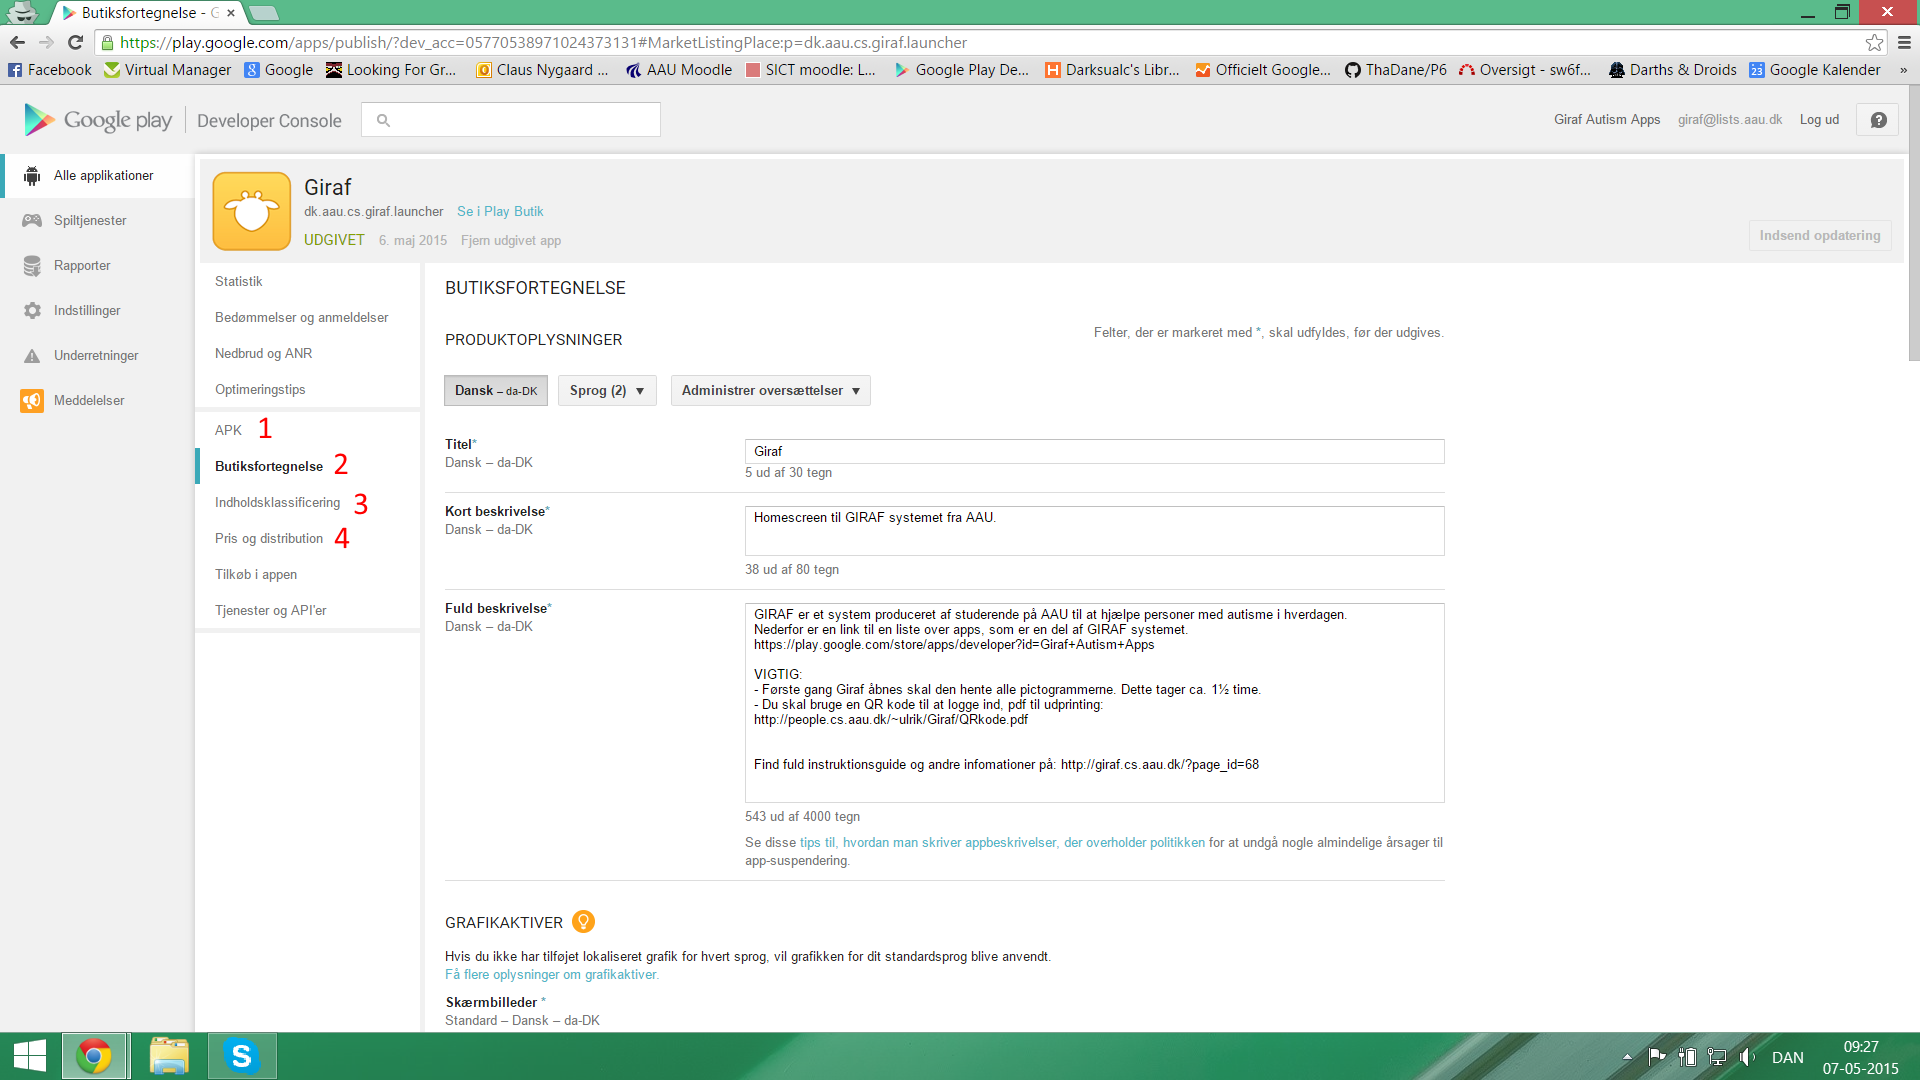
\includegraphics[width=0.8 \textwidth]{pictures/OverviewGooglePlay.png}
	\caption{Main page when logged in to Google analytics}
	\label{OverviewGooglePlay}
\end{figure}

Going to the APK-tab, see Figure \ref{VersionHandlingGooglePlay}, where all APKs for the app can be seen. This is separated into the production-version, a beta-version, and an alpha-version. The production-version is the one shown in Google Play, unless the one browsing the Play store are logged in on an account with test rights to the app. I.e. the production-version (1) might be 25, the beta-version (2) 28, and the alpha-version (3) could be 32. The alpha-version is alway newer than the beta-version which in turn is newer than the production-version. An alpha or a beta-version can be promoted to become the production-version, also the alpha-version can be promoted to become a beta-version (4).
It is also possible to change a previous version to be the active alpha, beta, or production-version, by first switching to the advanced state (5), and then click the button (6) to move it to the version needed.

\begin{figure}[H]
	\centering
	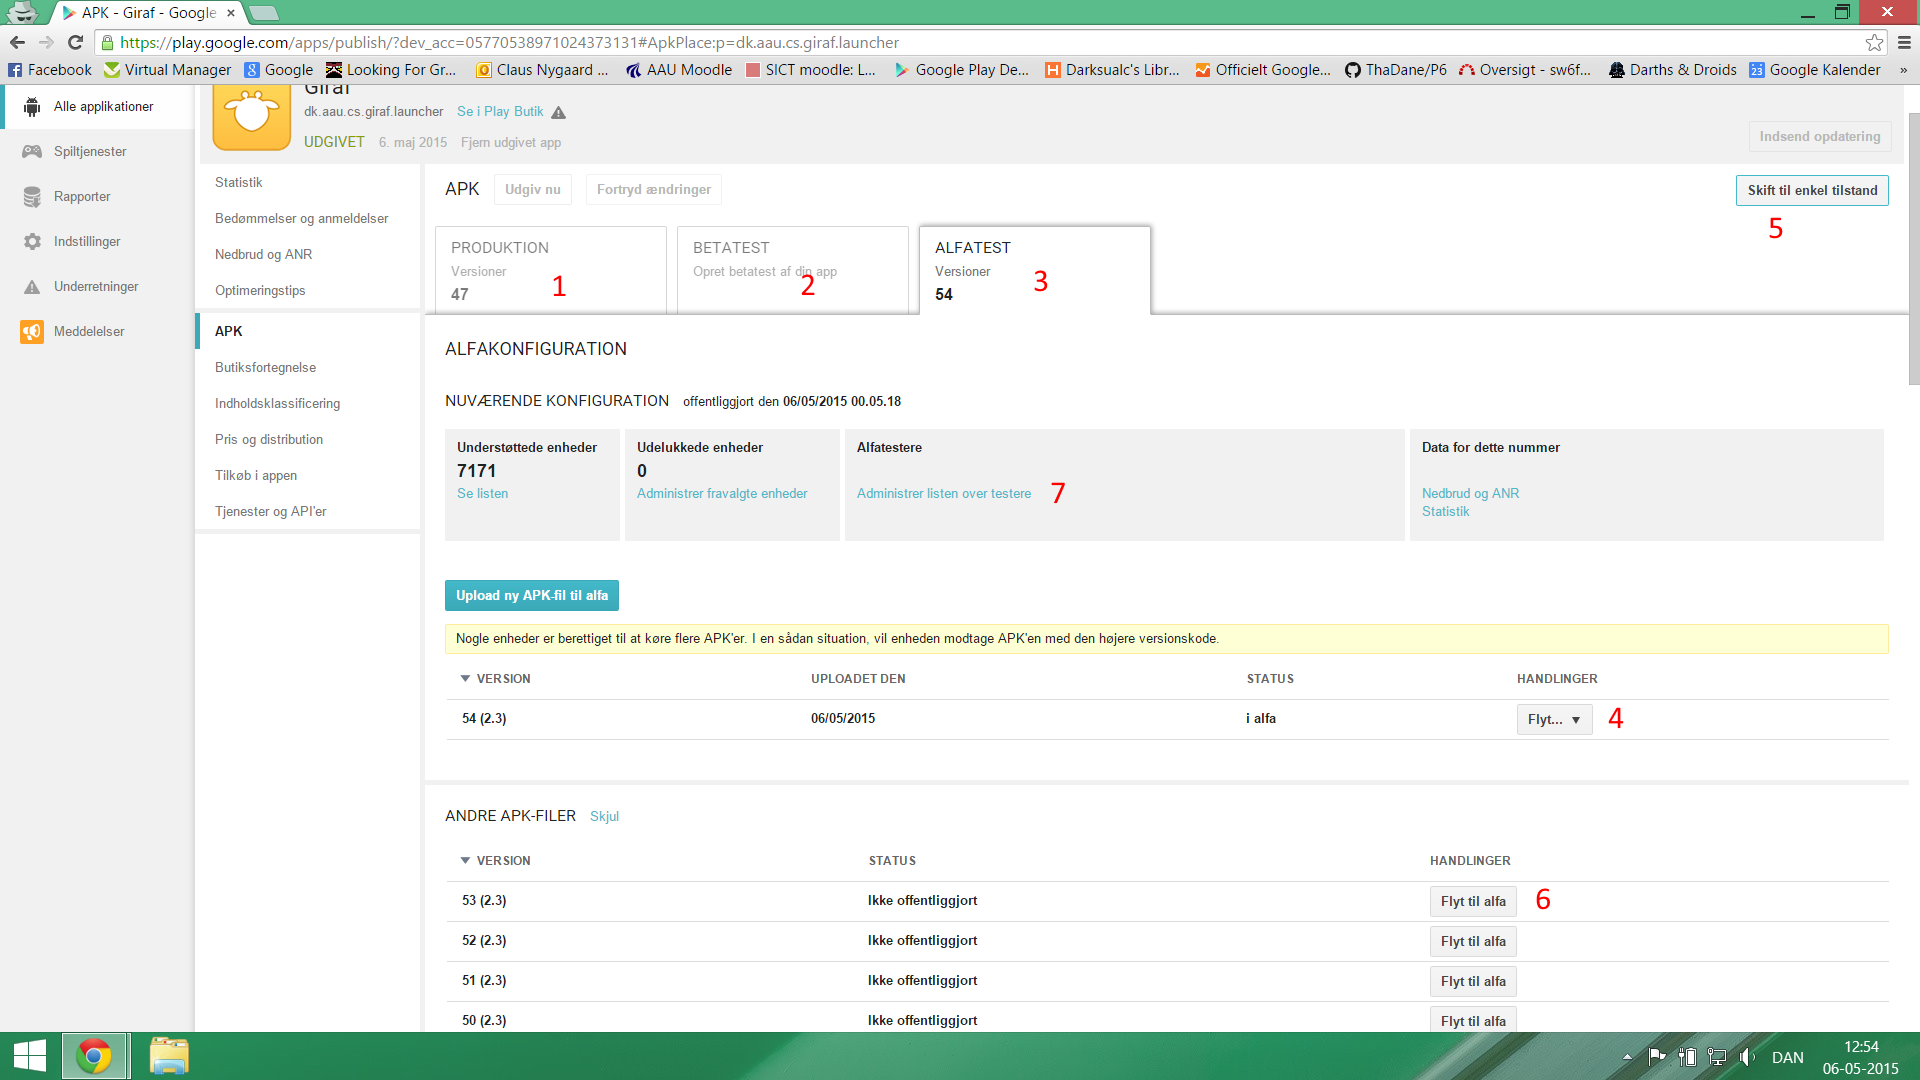
\includegraphics[width=0.8 \textwidth]{pictures/VersionHandlingGooglePlay.png}
	\caption{Main page when logged in to Google analytics}
	\label{VersionHandlingGooglePlay}
\end{figure}

\subsection{Giving access to alpha and beta-testing}
To give others access to alpha and beta versions, they need to be added to a Google Group that is assigned as a tester, either alpha or beta, on the app. The group ‘alfa-og-beta-testing-af-giraf@googlegroups.com’ was made for the purpose. When a person have been added to the group they will then have to go to ‘https://play.google.com/apps/testing/dk.aau.cs..giraf.PackageNameOfApp’ and accept to become tester on that app. Then if that person is logged in on a tablet, they will automatically download the alpha or beta-version of the app.
If a new app is added to Google Play, then the testing group will have to be added to the app as well. This is done by pressing the administrate the list of tester button (7) on Figure x.x, and then add the group.

Likewise there is a group specifically for beta testers, ‘beta-testing-af-giraf@googlegroups.com’, which grants beta versions but no alpha versions. The procedure for this group is identical to the other.
It is to be noted that it is only necessary to be a member of the first group, alfa-og-beta-testing-af-giraf, to have both alpha and beta testing available, though you will always use only the newest version, so if an alpha version is uploaded, then any beta version you are using will be replaced on the tablet.

\subsection{Content Classification} \label{Sprint4_SecContentClassification}
The content classification is a rating that shows which age groups are allowed to see the app in Google Play. In Denmark and the rest of Europe, except for Germany, the rating to follow is the PEGI-rating \citep{PEGI}. Google automatically assigns a rating to the app, after the developer, us, fills out a survey, where we declare what the app contains of content. Here it is important to distinguish between content that has been made by the developers and user-generated-content. The pictograms used in the apps we release can be counted as user-generated for the purpose of the content classification. This allows us to obtain a PEGI 3 rating, which means our apps are ‘safe for use’ by anyone from the age of three and upwards.